\documentclass[svgnames]{beamer}
\usepackage{mathpartir}
\usepackage{ulem}

\usecolortheme{orchid}
\setbeamertemplate{footline}[frame number]
\setbeamertemplate{navigation symbols}{}
\newcommand{\blue}[2]{{\color<{#1}>{blue}{#2}}}
\newcommand{\red}[2]{{\color<{#1}>{red}{#2}}}


\title{Verifying Event-Driven Programs using Ramified Frame Properties}

\author{Neelakantan R. Krishnaswami \texttt{<neelk@microsoft.com>} \\
        Lars Birkedal \texttt{<birkedal@itu.dk>} \\
        Jonathan Aldrich \texttt{<jonathan.aldrich@cs.cmu.edu>}}

\date{TLDI '10: 23 January 2010}

\newcommand{\ctext}[1]{\mbox{\textsf{{#1}}}}
\newcommand{\unittype}{\mathbf{1}}
\newcommand{\reftype}[1]{\ctext{ref }#1}
\newcommand{\monad}[1]{\bigcirc{#1}}
\newcommand{\cont}[1]{\ctext{cont}\;{#1}}
\newcommand{\opttype}[1]{\ctext{option }{#1}}
\newcommand{\seqsort}[1]{\ctext{seq }{#1}}
\newcommand{\listtype}[1]{\ctext{list }{#1}}

\newcommand{\pair}[2]{\left<{#1},{#2}\right>}
\newcommand{\fst}[1]{\ctext{fst } #1}
\newcommand{\snd}[1]{\ctext{snd } #1}

\newcommand{\inj}[1]{\iota_{#1}}
\newcommand{\inl}[1]{\ctext{inl }#1}
\newcommand{\inr}[1]{\ctext{inr }#1}
\newcommand{\Case}[5]{\ctext{case}(#1,\; {#2}.\; #3,\; {#4}.\; #5)}
\newcommand{\listcase}[5]{\ctext{case}(#1,\;\ctext{Nil} \to {#2},\;
                                       \ctext{Cons}({#3},{#4}) \to {#5})}
\newcommand{\Some}{\ctext{Some}}
\newcommand{\optcase}[4]{\ctext{case}(#1,\;
                                      \ctext{None} \to {#2},\;
                                      \ctext{Some}\;{#3} \to {#4})}
\newcommand{\z}{\ctext{z}}
\newcommand{\s}[1]{\ctext{s}(#1)}
\newcommand{\iter}[4]{\ctext{iter}(#1, {#2}, {#3}.\; {#4})}
\newcommand{\iterseq}[4]{\ctext{iter}_{\mathsf{seq}}(#1, {#2}, #3.\; {#4})}
\newcommand{\comp}[1]{[#1]}
\newcommand{\fun}[3]{\lambda #1:#2.\;#3}
\newcommand{\Fun}[3]{\Lambda #1:#2.\;#3}
\newcommand{\unit}{\left<\right>}
\newcommand{\pack}[2]{\ctext{pack}({#1}, {#2})}
\newcommand{\unpack}[4]{\ctext{unpack}({#1}, {#2}) = {#3} \;\ctext{in}\;{#4}}
% alt}{\;|\;}
% tv}[3]{\ctext{letv }#1 = #2\ctext{ in }#3}
% wref}[2]{\ctext{new}_{#1}(#2)}
% n}[1]{\ctext{run }{#1}}
% }{\ctext{ ok}}
% }[1]{\mathrm{FV}({#1})}
% 
% x}[2]{\ctext{fix}\;{#1}.\;{#2}}
% 
% atecfg}[2]{\left<{#1};\;{#2}\right>}
% al}[4]{\left<{#1};\;{#2}\right> \leadsto \left<{#3};\;{#4}\right>}
% alabort}[2]{\left<{#1};\;{#2}\right> \leadsto \mathbf{abort}}
% 
% main}[1]{\mbox{dom}({#1})}
% set}[1]{\mathcal{P}^{\uparrow}({#1})}
% 
% intsto}{\mapsto}
% sj}{\vee}
% implies}{\supset}
% nd}{-\!\!*}
% p}{\mathsf{emp}}
% lidprop}[1]{{#1}\ctext{ valid}}
% 
% do}[1]{\texttt{[TODO: {#1}]}}
% 
% tof}[1]{\{{#1}\}}
% 
% }{\Rightarrow}
% 
% {\mathbb{N}}
% 
% sert}{\ctext{prop}}
% 
% gstep}{\Downarrow}
% 
% geval}[4]{\left<{#1};\;{#2}\right> \bigstep \left<{#3};\;{#4}\right>}
% gevalabort}[2]{\left<{#1};\;{#2}\right> \bigstep \mathbf{abort}}
% 
% ec}[4]{\{{#1}\}{#2}\{{#3}.\;{#4}\}}
% ecX}[3]{\{{#1}\}{#2}\{{#3}\}}
% pec}[4]{\langle{#1}\rangle{#2}\langle{#3}.\;{#4}\rangle}
% falt}{\;\;|\;\;}
% 
% ecor}{\ctext{ or }}
% ecand}{\;\ctext{and}\;}
% ecimp}{\ctext{ implies }}
% ectype}{\ctext{spec}}
% lid}{\ctext{ valid}}
% 
% terp}[1]{[\![{#1}]\!]}
% terpE}[1]{\interp{#1}^e}
% terpC}[1]{\interp{#1}^c}
% 
% terpF}[1]{[\![{#1}]\!]_f}
% terpmono}[1]{\interp{#1}^{\mathrm{m}}}
% 
% tails}{\models}
% 
% dgeE}[4][\Theta]{{#1};\;{#2} \vdash {#3} : {#4}}
% dgeC}[4][\Theta]{{#1};\;{#2} \vdash {#3} \div {#4}}
% dgeEq}[5][\Theta]{{#1};\;{#2} \vdash {#3} \equiv {#4} : {#5}}
% dgeEqC}[5][\Theta]{{#1};{#2} \vdash {#3} \equiv {#4} \div {#5}}
% 
% 
% 
% 
% rations
% 
% mfun}[2]{\lambda #1.\;#2}
% mpair}[2]{\left({#1}, {#2}\right)}
% werset}[1]{\mathcal{P}(#1)}
% 
% ircat}[2]{\left<{#1};{#2}\right>}
% mcat}[2]{\left[{#1};{#2}\right]}
% scat}[1]{\lambda({#1})}
% 
% 
% dgeP}[3]{{#1} \vdash {#2} : {#3}}
% dgeS}[2]{{#1} \vdash {#2} : \spectype}
% 
% dgeSCtx}[2]{{#1} \vdash {#2} : \ctext{context}}
% 
% dgeEqP}[4]{{#1} \vdash {#2} \equiv {#3} : {#4}}
% 
% 
% dgeWK}[3][\Theta]{{#1} \vdash {#2} : {#3}}
% dgeKeq}[4][\Theta]{{#1} \vdash {#2} \equiv {#3} : {#4}}
% 
% tailsP}[3]{{#1} \rhd {#2} \vdash {#3}}
% tailsS}[3]{{#1}; {#2} \vdash {#3} \ok}
% 
% artp}{\ctext{char}}
% nttp}{\ctext{font}}
% 
% C}{loc}
% NO}{\mathbf{mono}}
% AP}{heap}
% OP}{Prop}
% UE}{True}
% ROP}{Prop}
% PE}{Type}
% 
% p}{Proposition}
% emma}{Lemma}
% 
% t{proof}{\noindent\textbf{Proof (Sketch).}}{\noindent$\Box$}
% 
% {tabbedproof}{\begin{tabbing}\;\;\=\;\;\=\;\;\=\;\;\=\;\;\=\;\;\=\;\;\=\;\;\=\\[-2em]}{\end{tabbing}}
% 
% }{\>}
% o}{\>\>}
% oo}{\>\>\>}
% ooo}{\>\>\>\>}
% oooo}{\>\>\>\>\>}
% ooooo}{\>\>\>\>\>\>}
% oooooo}{\>\>\>\>\>\>\>}
% ooooooo}{\>\>\>\>\>\>\>\>}
% 
% 
% {eqnproof}[1][]{${#1}$\begin{displaymath}\begin{array}{lcll}}
%           {\end{array}\end{displaymath}}
% 
% 
% ine}[3][]{{#1} & = & {#2} & \mbox{{#3}} \\}
% 
% ines}[3][]{{#1} & = & \begin{array}{l} #2 \end{array} & \mbox{{#3}} \\}
% 
% laim}[3][]{{#1} &  & {#2} & \mbox{{#3}} \\}
% act}[2]{{#1} & & & \mbox{#2} \\}
% 
%%

\newcommand{\runcmd}{\ctext{run}\;}
\newcommand{\return}{\ctext{return}\;}
\newcommand{\bind}{\ctext{bind}\;}
\newcommand{\readcell}{\ctext{read}\;}


\newcommand{\ready}[3]{\ctext{ready}({#1}, {#2}, {#3})}
\newcommand{\unready}[2]{\ctext{unready}({#1}, {#2})}

\newcommand{\cellprop}[5]{\ctext{cell}^{#1}({#2}, {#3}, {#4}, {#5})}
\newcommand{\cellneg}[2]{\cellprop{-}{#1}{#2}{\_}{\_}}
\newcommand{\cellpos}[4]{\cellprop{+}{#1}{#2}{#3}{#4}}
\newcommand{\celleither}[2]{\cellprop{\pm}{#1}{#2}{-}{-}}
\newcommand{\localref}[2]{\ctext{local}({#1}, {#2})}
\newcommand{\localstate}{\mathit{localstate}}
\newcommand{\getref}{\ctext{getref}\;}
\newcommand{\setref}{\ctext{setref}\;}

\newcommand{\aconfig}[2]{\left<{#1};{#2}\right>}
\newcommand{\aeffect}[2]{\left[{#1}|{#2}\right]}
\newcommand{\astep}[6]{\aconfig{#1}{#2}\Downarrow\aconfig{#3}{#4}\aeffect{#5}{#6}}

\newcommand{\powersetfin}[1]{\mathcal{P}^{\mathrm{fin}}({#1})}
\newcommand{\celltype}[1]{\ctext{cell}\;{#1}}
\newcommand{\bool}{\ctext{bool}}
\newcommand{\settype}[1]{\ctext{Set}({#1})}

\newcommand{\codetype}[1]{\ctext{code}\;{#1}}

\newcommand{\newcell}{\ctext{newcell}\;}
\newcommand{\cellset}{\ctext{cellset}}
\newcommand{\addset}{\ctext{addset}}

\newcommand{\comprehend}[2]{\setof{{#1}\;|\;{#2}}}
\newcommand{\ST}[2]{\ctext{ST}({#1}, {#2})}
\newcommand{\stream}[1]{\ctext{stream}({#1})}
\newcommand{\formula}{\ctext{formula}}


\newcommand{\updatecell}{\ctext{update}}


\newcommand{\liftop}{\ctext{lift}\;}
\newcommand{\seqop}{\ctext{seq}\;}
\newcommand{\parop}{\ctext{par}\;}
\newcommand{\loopop}{\ctext{loop}\;}
\newcommand{\switchop}{\ctext{switch}\;}

\newcommand{\satisfies}[2]{\mathit{satisfies}({#1}, {#2})}
\newcommand{\sat}{\mathit{sat}}

\newcommand{\closed}[2]{\ctext{closed}({#1}, {#2})}

\newcounter{spec:linenum}

\newenvironment{specification}
               {\setcounter{spec:linenum}{0}
                \begin{tabbing}
                  \qquad \= \\[-2em]}
               {\end{tabbing}}

\newcommand{\nextline}[1][0em]{\refstepcounter{spec:linenum}\\[#1]\arabic{spec:linenum} \>}
\newcommand{\nextlinelabel}[2][0em]{\refstepcounter{spec:linenum}\label{#2}\\[#1]\arabic{spec:linenum} \>}

\newcommand{\lifttrans}{\mathit{lift}}
\newcommand{\seqtrans}{\mathit{seq}}
\newcommand{\partrans}{\mathit{par}}
\newcommand{\switchtrans}{\mathit{switch}}
\newcommand{\looptrans}{\mathit{loop}}
\newcommand{\cycletrans}{\mathit{cycle}}
\newcommand{\gentrans}{\mathit{gen}}
\newcommand{\maptrans}{\mathit{map}}


\begin{document}
\begin{frame}
  \titlepage
\end{frame}

\section{Introduction}

\begin{frame}
  \frametitle{The Question}

    \begin{itemize}
      \item Separation logic permits local reasoning\ldots \pause
      \item \ldots\ but what happens when our invariants are global? \pause
    \end{itemize}

  \begin{block}{Our (Partial) Answer}
    \begin{itemize}
      \pause\item Structure the global invariant to permit some local reasoning
      \pause\item Use a \emph{ramification operator} to summarize global effects
      \pause\item Illustrated with a case study from event-driven programming
    \end{itemize}
  \end{block}
\end{frame}

\begin{frame}
  \frametitle{Outline}
  \tableofcontents
\end{frame}

\section{Our Language and Logic}

%%
\begin{frame}
  \frametitle{What Is Separation Logic?}

%  \begin{block}{}
    \begin{itemize}
      \item Extension of Hoare logic to simplify reasoning about aliased data
      \item Adds \emph{separating conjunction} $P * Q$ in addition 
        to $P \land Q$
        \begin{center}
        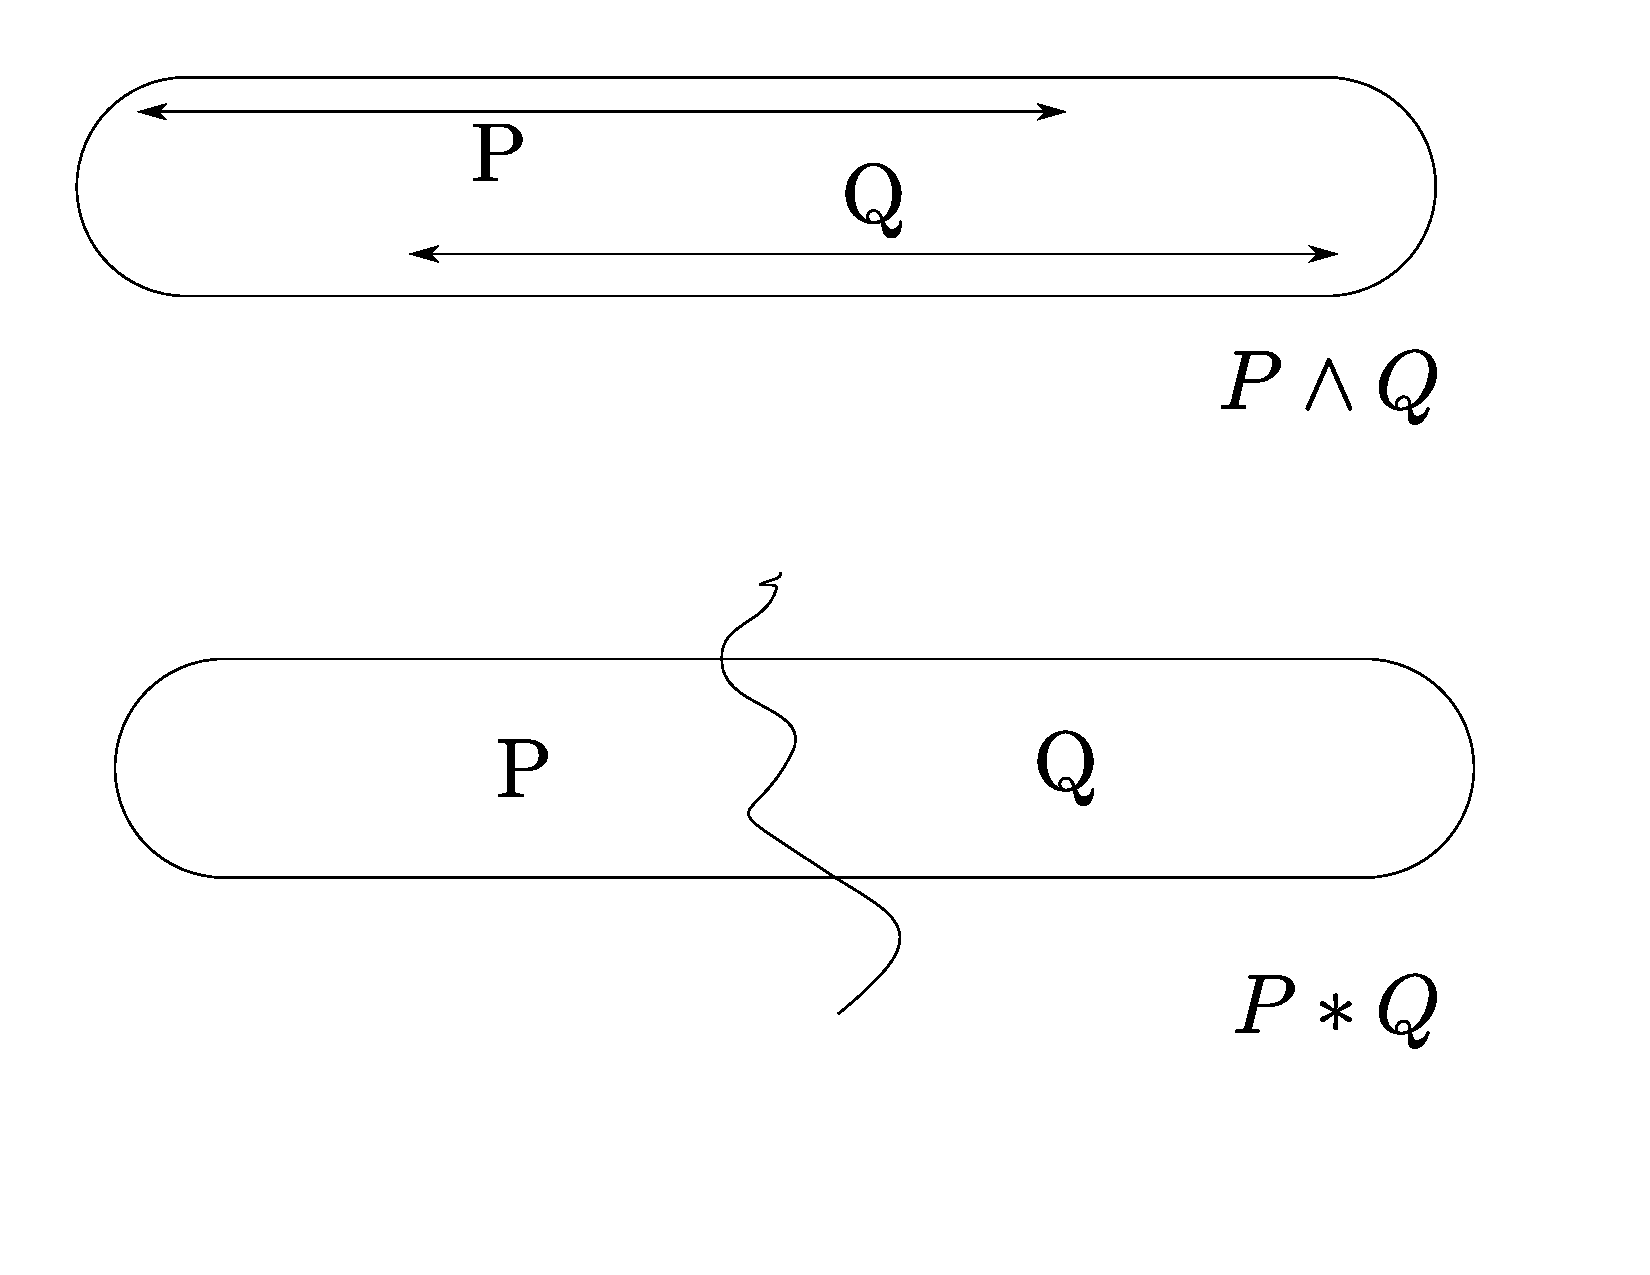
\includegraphics[height=1.5in]{separating-conjunction.pdf}
        \end{center}
      \item Very successful: garbage collectors and device drivers
      \item \pause But high-level programs have aliasing bugs too!
    \end{itemize}
%  \end{block}
\end{frame}

%%
\begin{frame}
\frametitle{Our Programming Language}

\begin{block}{Types}
\begin{displaymath}
 \begin{array}{llcl}
    A & ::= & b \bnfalt A \to B \bnfalt \monad{A} \bnfalt \ctext{ref}A 
   \bnfalt  \forall \alpha.\;A \bnfalt \exists \alpha.\;A \bnfalt \alpha \\
  \end{array}
\end{displaymath}
\end{block}

%\begin{block}{Features}
\begin{itemize}
  \item Core: pure typed lambda-calculus plus polymorphism
  \item All effects (state, nontermination) encapsulated in monad $\monad{A}$
  \item Denotational model, validates $\beta\eta$-equalities
\end{itemize}
%\end{block}
\end{frame}

%%
\begin{frame}
  \frametitle{Specifications}
  
 % \begin{block}{}
    \begin{itemize}
    \item Hoare triples on computation terms of type $\bigcirc{A}$:

      \begin{center}$\specX{P}{e}{r:A.\;Q}$
      \end{center}

      \begin{itemize}
        \item $P$ -- precondition state
        \item $e$ -- monadic command to run
        \item $Q$ -- postcondition
        \item $r:A$ -- binder for return value
      \end{itemize}

    \item Triples are atoms of a logic of specifications (Reynolds 1981)

    \item Supports \emph{frame rule}: 
      \begin{mathpar}
        \inferrule*[]
                  { \specX{P}{e}{r:A.\;Q} }
                  { \specX{P*F}{e}{r:A.\;Q*F} }
      \end{mathpar}

  \end{itemize}

\end{frame}
 
% %%
\begin{frame}
  \frametitle{Assertion Logic}

    \begin{itemize}
      \item All usual logical connectives, plus spatial connectives: 

        \begin{center}$P * Q$, $e \pointsto e'$, etc.
        \end{center}

      \item Supports higher-order quantification: 

        \[\exists P:\assert. Q\]

      \item Essential for information hiding and modularity

        \[counter(c, 17)\]

      \item Model of $\assert$ is usual powerset model of heaps (Biering \emph{et al} 2005)
    \end{itemize}
\end{frame}


\begin{frame}
  \frametitle{Talk Outline}
%  \begin{block}{}
  \begin{itemize}
    \item The Low Level 
      \begin{itemize}
        \item Imperative Notification: Pointers, Heaps, and Graphs, oh my!
      \end{itemize}
    \item The \sout{Messy} Elegant Middle
      \begin{itemize}
        \item An abstract semantics for imperative notification networks
        \item Relating the low and the middle
      \end{itemize}
    \item Up to the High Level    \item Related Work
  \end{itemize}
% \end{block}
\end{frame}

%   \section{The High Level Specification}
%   \subsection{What is a specification for a GUI?}
%   %%
%   \begin{frame}
%     \frametitle{Functional Reactive Programming} 
%     
%   %  \begin{block}{}
%     \begin{itemize}
%       \item We use \emph{Functional Reactive Programming} to specify GUIs
%       \item View interactive programs as stream transducers
%     \end{itemize}
%   %  \end{block}
%   
%     \pause
%   
%   %  \begin{block}{}
%       \begin{itemize}
%         \item Transducer type: $ST(A,B) \equiv Stream(A) \to Stream(B)$
%         \item $Stream(A) \equiv \mathsf{Time} \to A$
%         \item Simple, well-behaved mathematical characterization 
%       \end{itemize}
%   %  \end{block}
%   \end{frame}
%   
%   %%
%   \begin{frame}
%     \frametitle{Functional Reactive Programming in a Nutshell}
%     \begin{center}
%       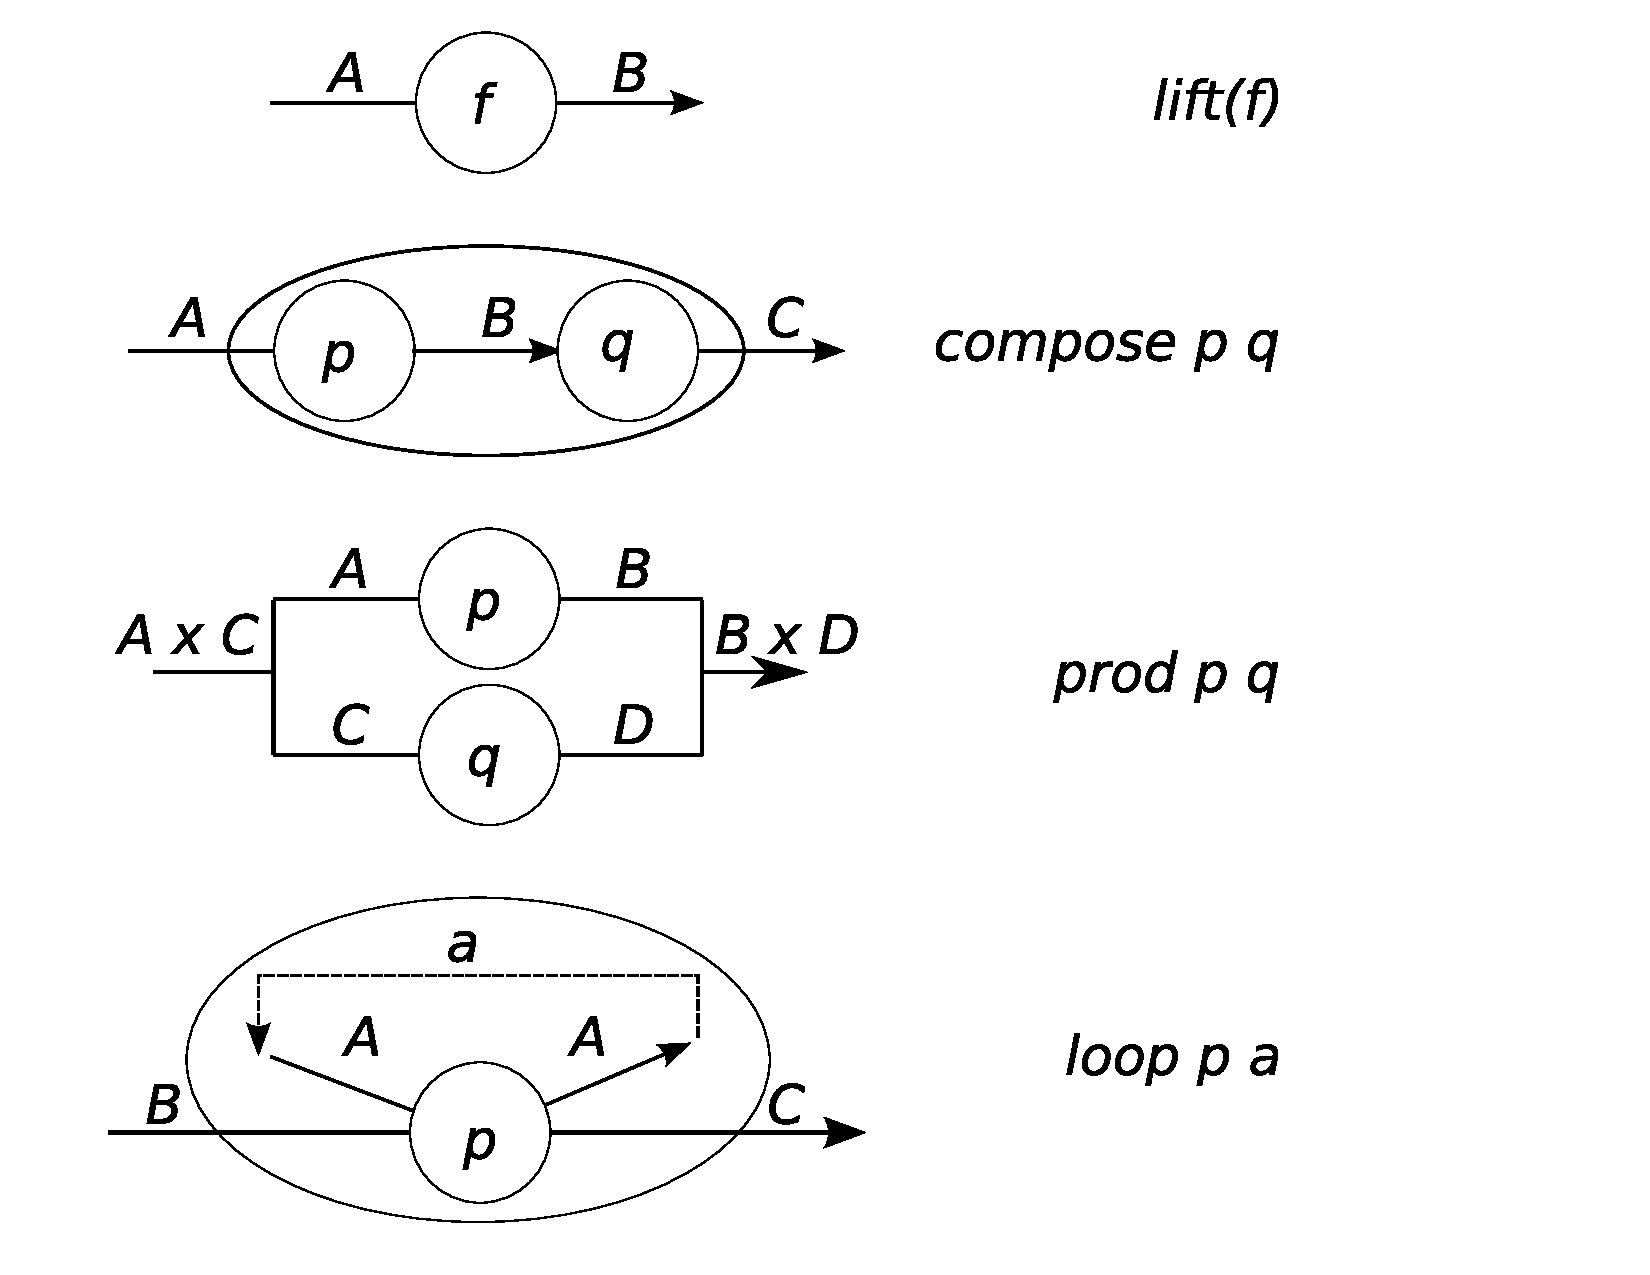
\includegraphics[height=3in]{frp-picture.pdf}
%     \end{center}
%   \end{frame}
%   
%   %%
%   \begin{frame}
%     \frametitle{Why FRP is (and isn't) a Good Fit for GUIs}
%   
%   %  \begin{block}{Dataflow in a Model-View Controller Architecture}
%       \begin{center}
%       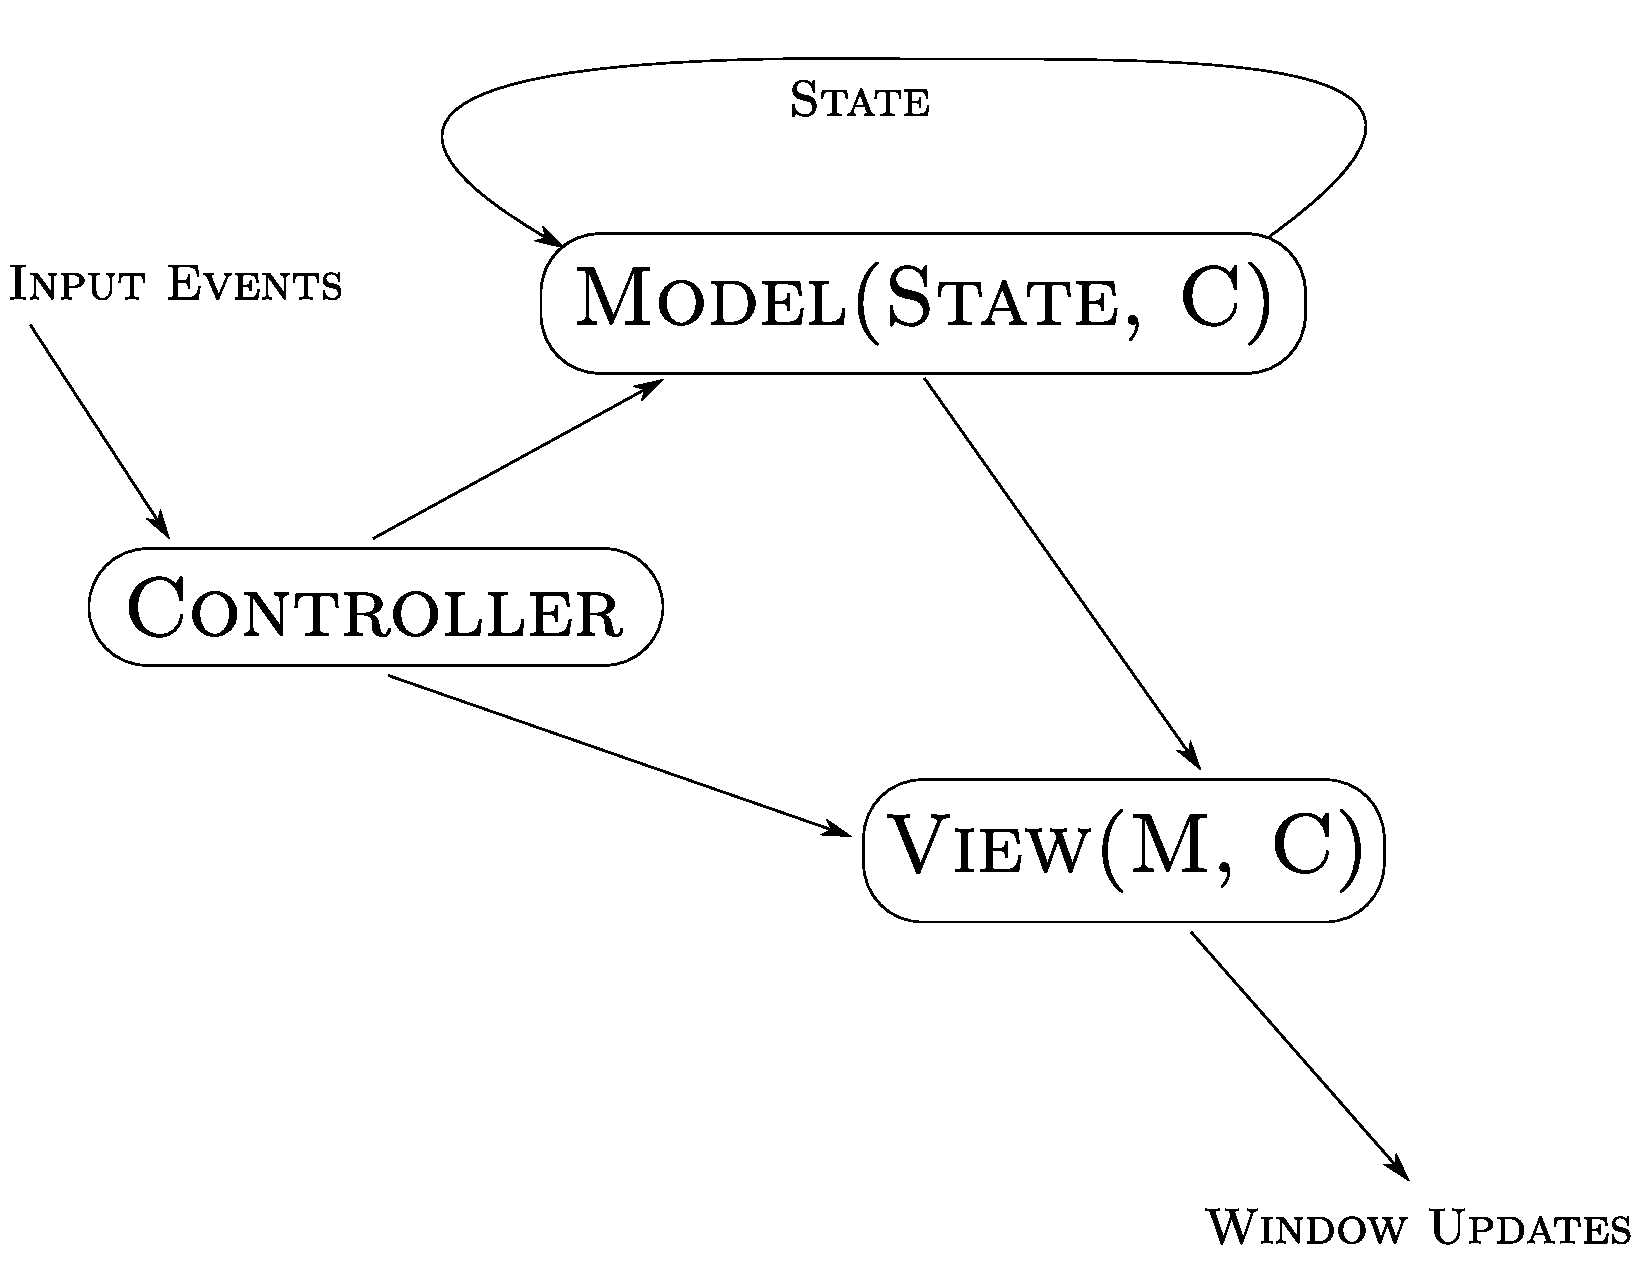
\includegraphics[height=2in]{mvc.pdf}
%       \end{center}
%   %  \end{block}
%   
%     \begin{center}A \emph{GUI} is an $ST(Event, Window)$! (Courtney 2003)    
%     \end{center}
%   \end{frame}
%   
%   %%
%   \subsection{Proof Structure}
%   \begin{frame}
%     \frametitle{The Overall Architecture of the Proof}
%     \begin{center}
%     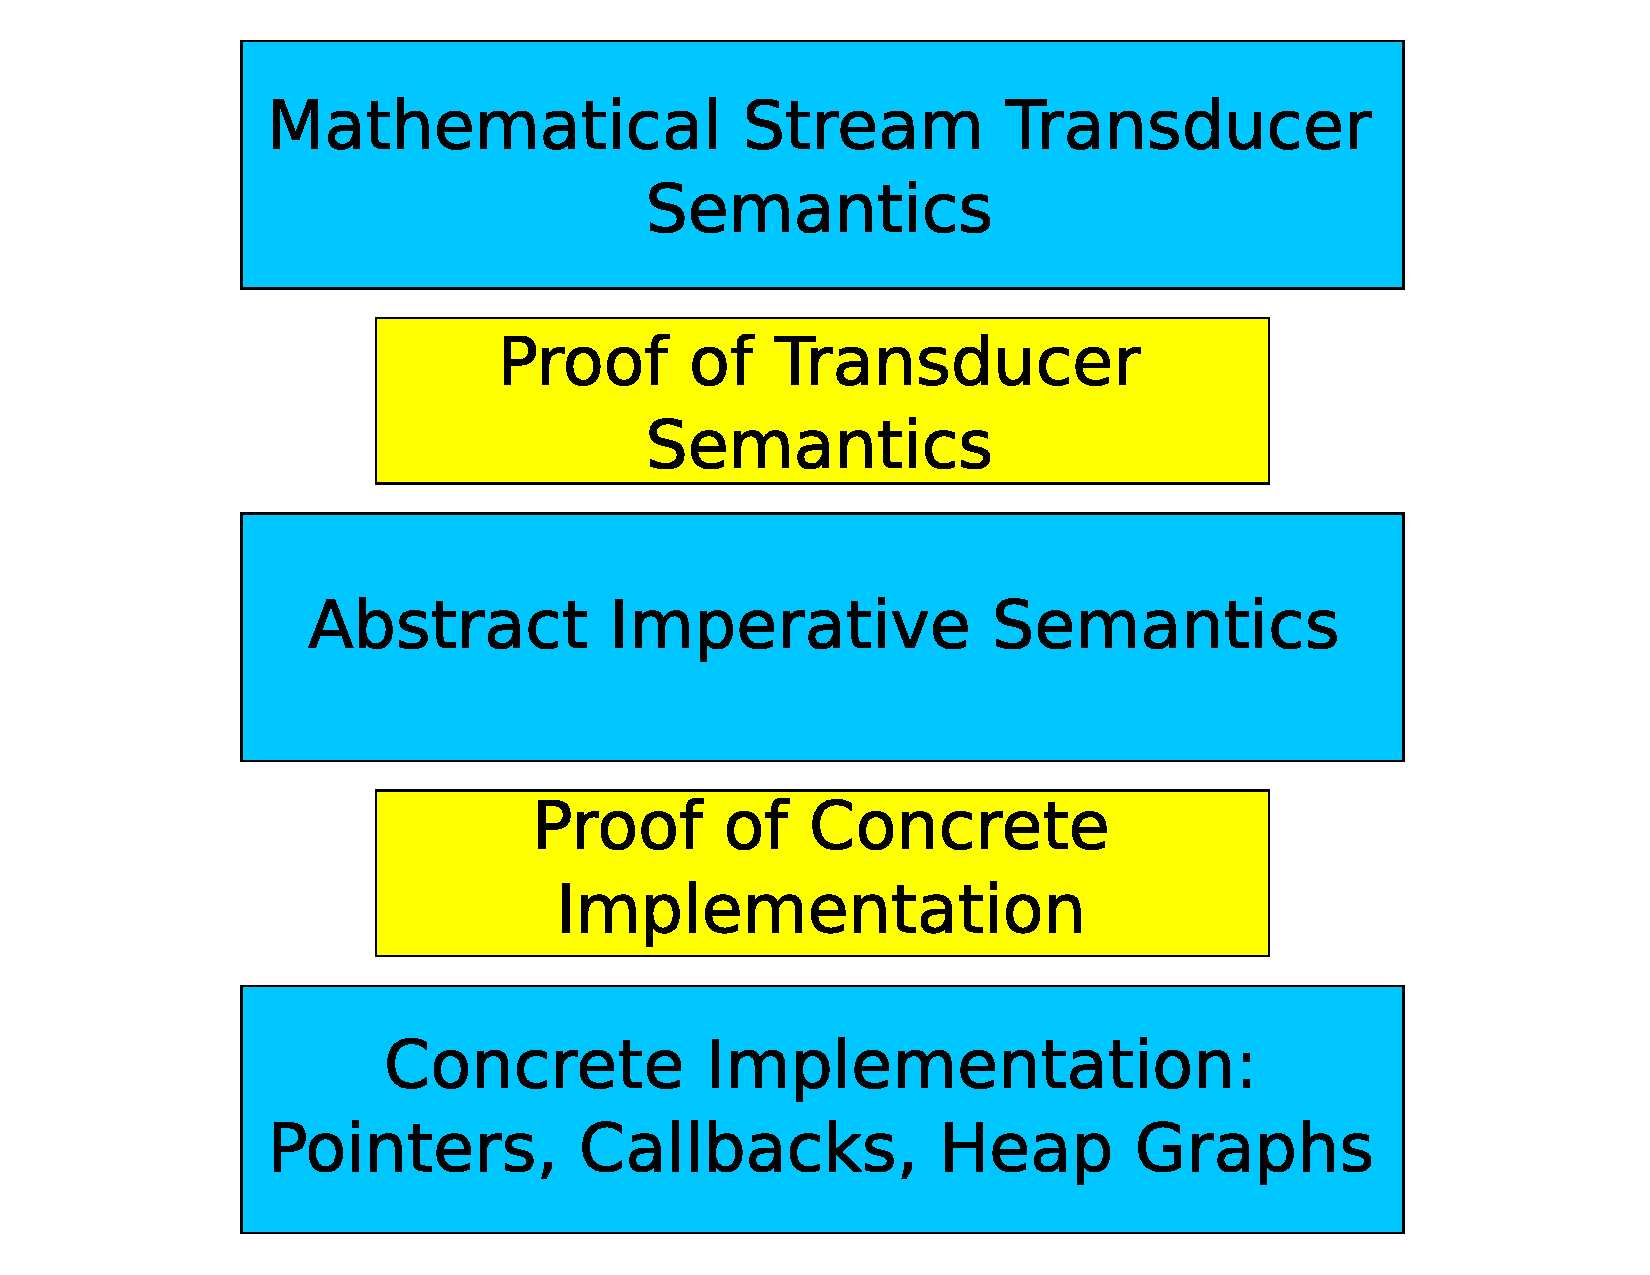
\includegraphics[height=3in]{proof-structure.pdf}
%     \end{center}
%   \end{frame}

%%
\begin{frame}
  \frametitle{Talk Outline}
%  \begin{block}{}
  \begin{itemize}
      
    \item \blue{1-}{The Low Level}
      \begin{itemize}
        \item Imperative Notification: Pointers, Heaps, and Graphs, oh my!
      \end{itemize}

    \item The \sout{Messy} Elegant Middle
      \begin{itemize}
        \item An abstract semantics for imperative notification networks
        \item Relating the low and the middle
      \end{itemize}
    \item Up to the High Level    \item Related Work
  \end{itemize}
%  \end{block}
\end{frame}

\section{The Low Level Implementation}

% %%
% \begin{frame}
%   \frametitle{Model-View Controller Revisited}
% 
%   \begin{block}{}
%     \begin{center}
%     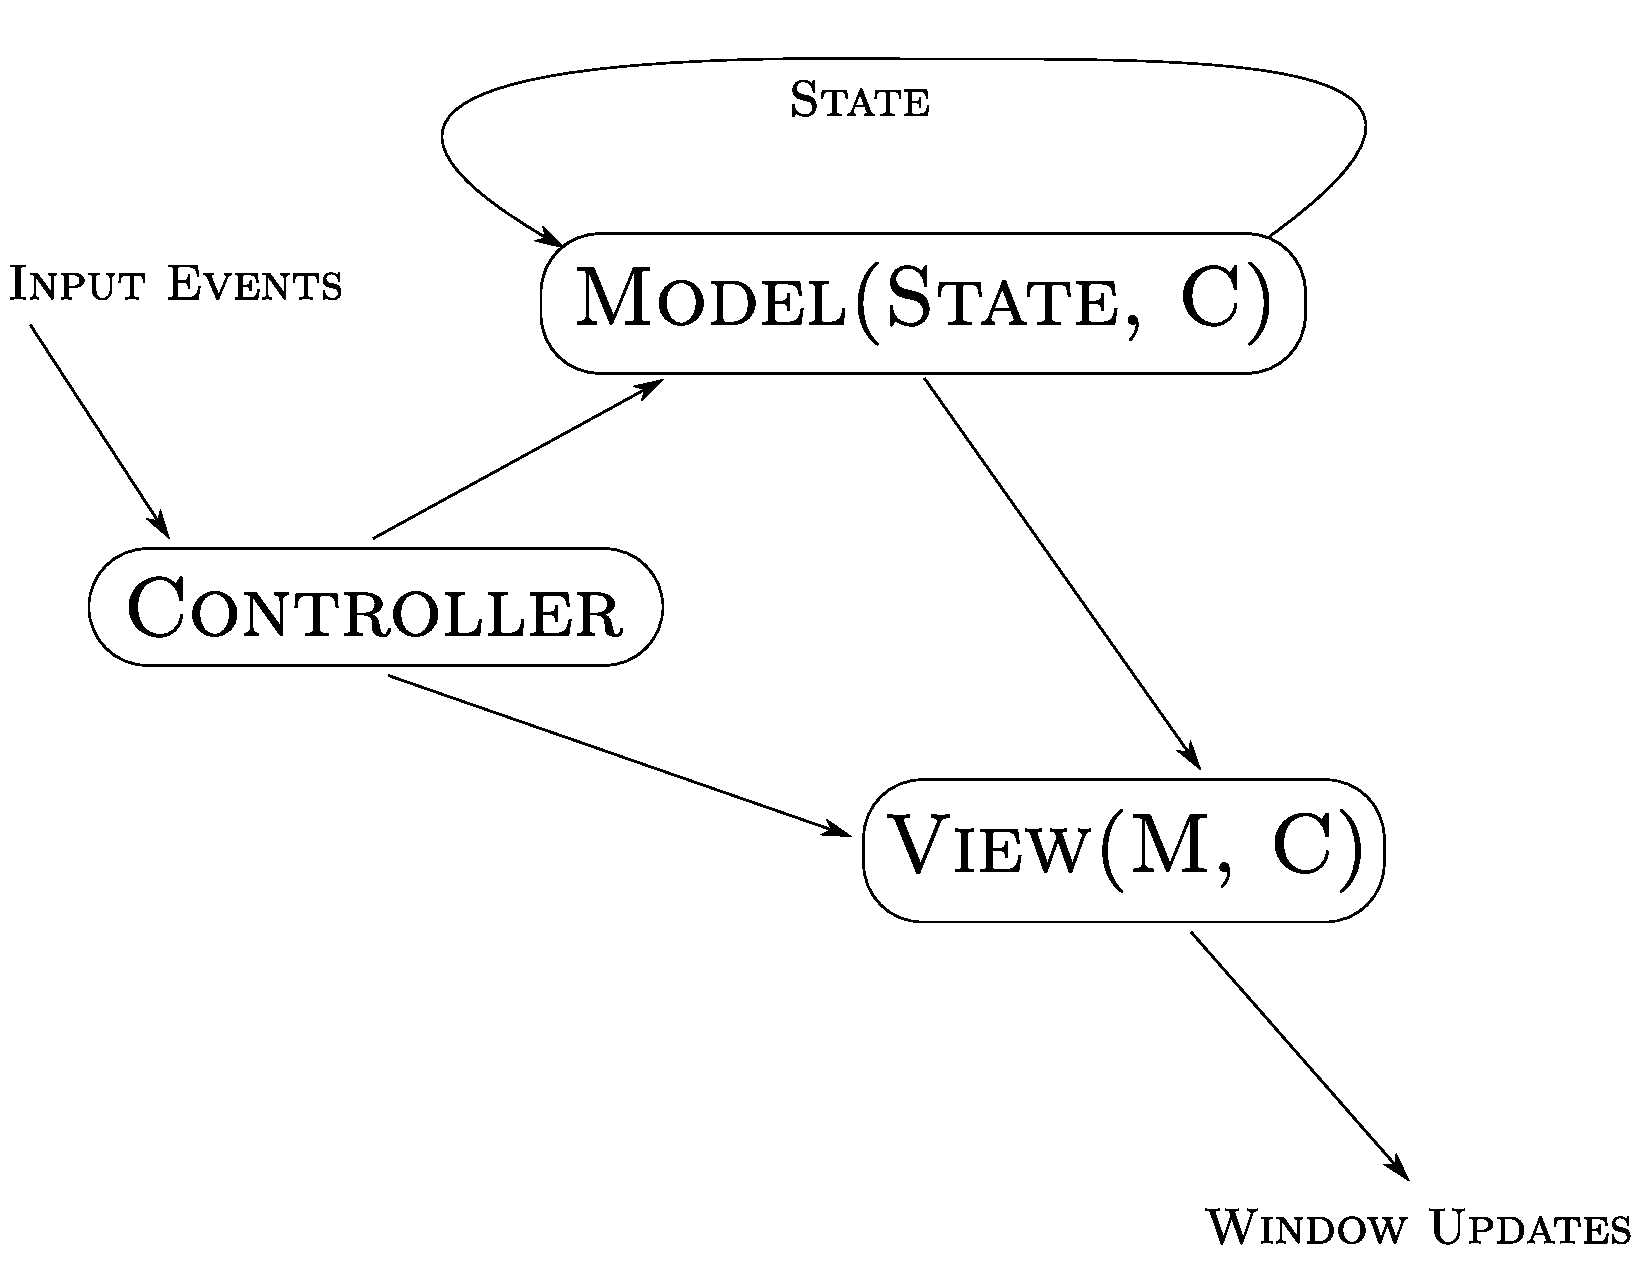
\includegraphics[height=2in]{mvc.pdf}
%     \end{center}
%   \end{block}
% 
%   \begin{itemize}
%   \item Notifications require dependencies
%   \item Model gives itself to controller, view to model and controller
%   \end{itemize}
% \end{frame}


%%
\begin{frame}[fragile]
  \frametitle{Imperative Notification Interface}

  $T(A)$ monadic type built from language's pre-existing state monad
  \begin{block}{}
  \begin{semiverbatim}
    T(A) = \(\bigcirc\)(A \(\times\) Set(anycell))
 
    return : \(\alpha\) \(\to\) T(\(\alpha\))
    bind   : T(\(\alpha\)) \(\to\) (\(\alpha\) \(\to\) T(\(\beta\))) \(\to\) T(\(\beta\))
    read   : Cell(\(\alpha\)) \(\to\) T(\(\alpha\))

    update : Cell(\(\alpha\)) \(\to\) T(\(\alpha\)) \(\to\) \(\bigcirc(1)\)
  \end{semiverbatim}
%    getref : ref \(\alpha\) \(\to\) T(\(\alpha\)) 
%    setref : ref \(\alpha\) \(\to\) \(\alpha\) \(\to\) T(1) 
  \end{block}
  \begin{itemize}
    \item Computations of type $T(A)$:
      \indent\begin{itemize} 
        \item compute a value of type $A$, and
        \item returns all of the cells that it directly read
      \end{itemize}

    \item Implementation manages dependencies
  \end{itemize}
\end{frame}


%%
\begin{frame}
  \frametitle{Imperative Notification Networks}

  \includegraphics<1>[height=3in]{dependency-graph.pdf}
  \includegraphics<2>[height=3in]{dependency-graph-1.pdf}
  \includegraphics<3>[height=3in]{dependency-graph-2.pdf}
  \includegraphics<4>[height=3in]{dependency-graph-3.pdf}
  \includegraphics<5>[height=3in]{dependency-graph-4.pdf}
  \includegraphics<6>[height=3in]{dependency-graph-5.pdf}
  \includegraphics<7>[height=3in]{dependency-graph-6.pdf}
\end{frame}

%%
\begin{frame}[fragile]
  \frametitle{Implementing Cells}
  \begin{block}{}
  \begin{semiverbatim}
    Cell(\(\alpha\)) = \{
      value:     ref option(\(\alpha\));     
      expr:      ref T(\(\alpha\));          
      sources:   ref Set(anycell);  
      observers: ref Set(anycell)   
    \}

    anycell = \(\exists\;\alpha.\) Cell(\(\alpha\))
  \end{semiverbatim}
  \end{block}
  \begin{itemize}
  \item \texttt{read} checks \texttt{value} field, may reevaluate \texttt{expr} and set \texttt{sources}
  \item \texttt{update} modifes \texttt{expr}, \texttt{value}, and transitively invalidates \texttt{observers}
  \end{itemize}
\end{frame}


%%
\begin{frame}
  \frametitle{Low-Level Heap Invariants}

%  \begin{block}{What Makes Verifying This Hard?}
    \begin{itemize}
      \item Invariants: 
        \begin{itemize}
        \item Valid nodes must be acyclic
        \item Valid nodes cannot have invalid nodes in \texttt{read}
        \item If $c'$ in \texttt{sources} of $c$, then $c$ in \texttt{observers} of $c'$
        \end{itemize}

    \item Imposes \emph{global} consistency invariants on the heap's 
      graph structure

    \item However, we need \emph{local} reasoning principles

      We want to verify independent parts of the network independently
    \end{itemize}
%  \end{block}
\end{frame}


\section{The Middle Level}
%%
\begin{frame}
  \frametitle{Talk Outline}
%  \begin{block}{}
  \begin{itemize}
      
    \item The Low Level
      \begin{itemize}
        \item Imperative Notification: Pointers, Heaps, and Graphs, oh my!
      \end{itemize}
    \item \blue{1-}{The \sout{Messy} Elegant Middle}
      \begin{itemize}
        \item An abstract semantics for imperative notification networks
        \item Relating the low and the middle
      \end{itemize}
    \item Up to the High Level    \item Related Work
  \end{itemize}
%  \end{block}
\end{frame}

%%
\begin{frame}
  \frametitle{Abstract Properties of the Low-Level Interface}

  The Problem:
%  \begin{block}{The Problem}
    \begin{itemize}
      \item Implementations of $T(A)$ requires knowing the whole
        notification graph
        
      \item Arises because of symmetry of \texttt{sources} and 
        \texttt{observers}
    \end{itemize}
%  \end{block}

  \pause
%  \begin{block}{The Solution!}
  \ \\
  The Solution:
    \begin{itemize}
      \item Find an abstraction of the network: hide half of 
        the dependency graph
        
        \ \\ 
      \item Give an abstract semantics for commands of type $T(A)$ via 
        abstract heap
    \end{itemize}
%  \end{block}
\end{frame}

\subsection{Abstracting the Notification Network}
%%
\begin{frame}
  \frametitle{Abstract Heap Descriptions}

%  \begin{block}{}
  \begin{displaymath}
    \begin{array}{lcll}
      \phi & ::= & I                    & \mbox{Empty Network} \\
           &  |  & \phi \otimes \psi    & \mbox{Disjoint Combination} \\ 
           &  |  & \cellbad{a}{e}       & \mbox{Un-ready Cell} \\
           &  |  & \cellok{a}{e}{v}{src} & \mbox{Possibly-Ready Cell} \\
    \end{array}
  \end{displaymath}
%  \end{block}

  \ \\

  \begin{itemize}
    \item \pause Notice that only \texttt{sources} kept in description
    \item \pause Will prove essential for local reasoning
    \item \pause Cells have may/must flavor
  \end{itemize}
\end{frame}

%%
\begin{frame}
  \frametitle{How Readiness Propagates}

  \begin{center}
  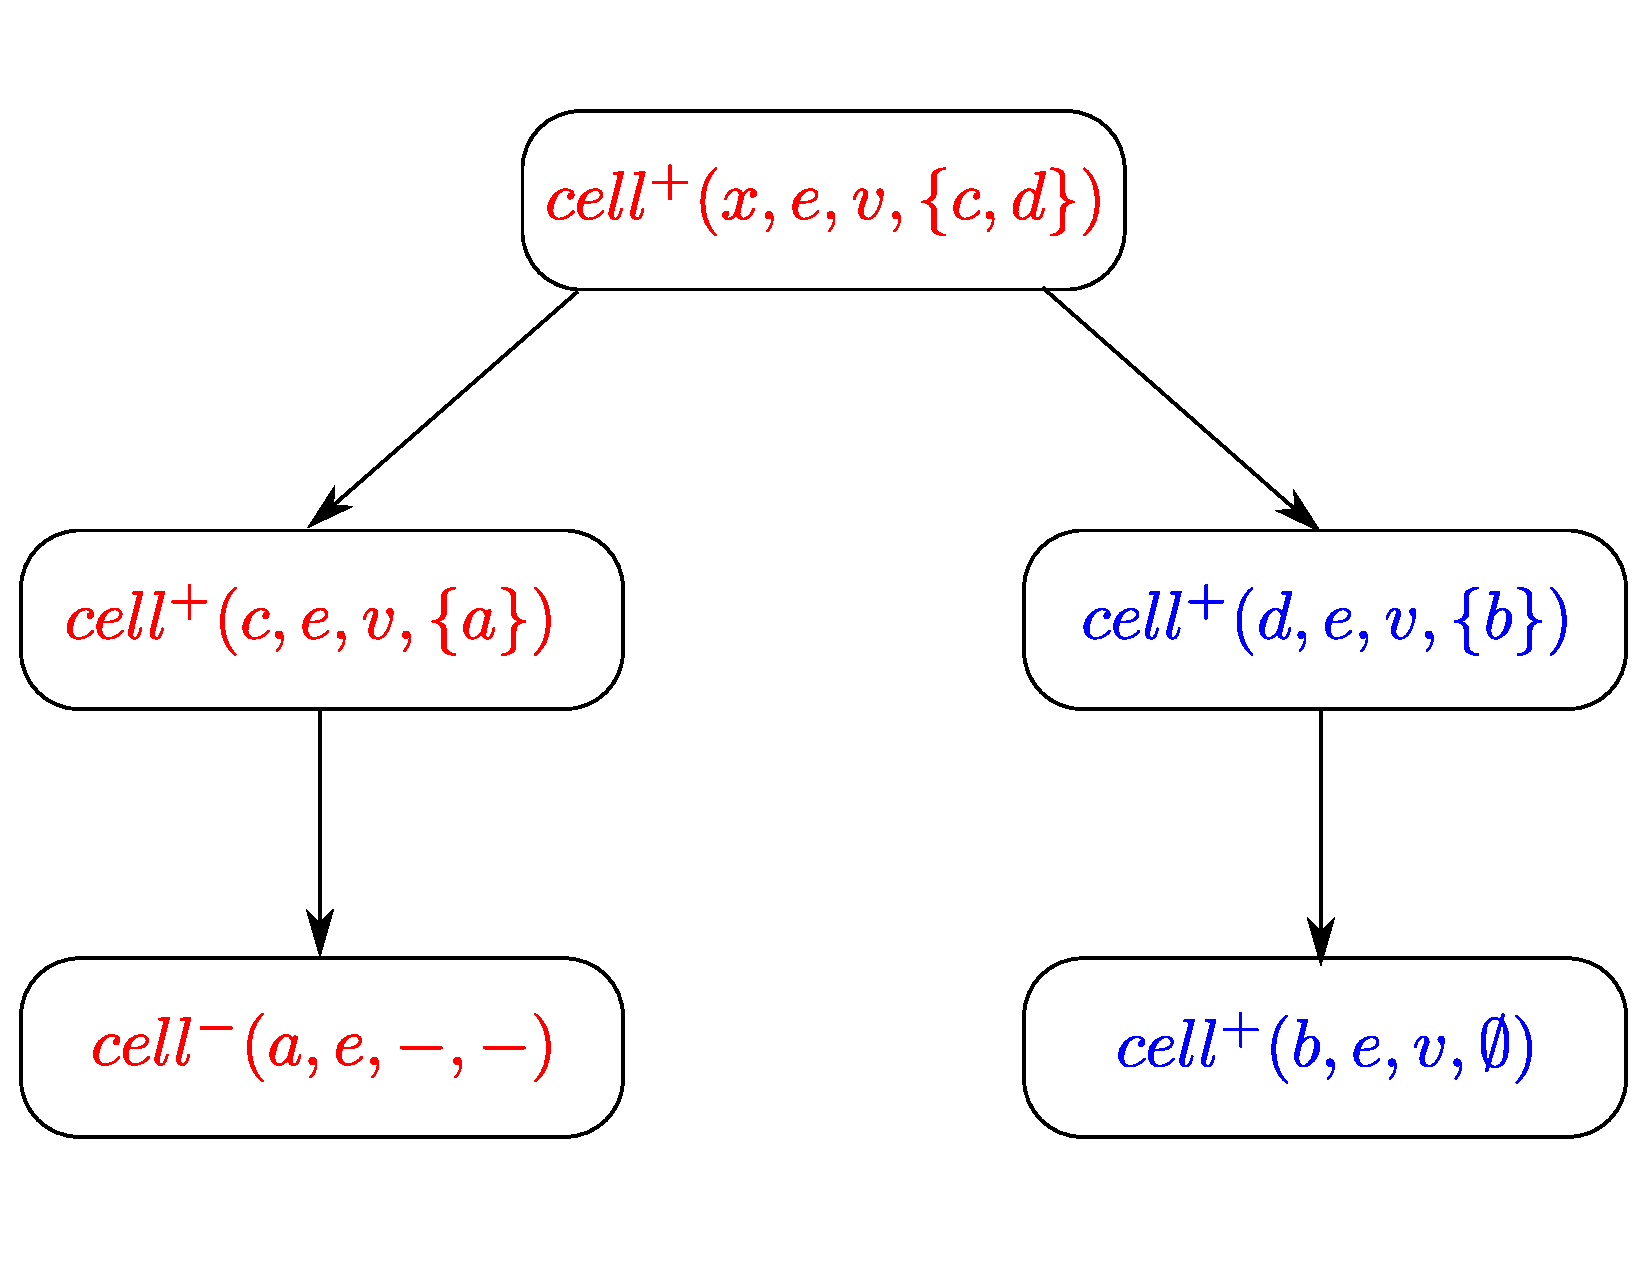
\includegraphics[height=2.5in]{conditional-validity-0.pdf}
  \end{center}

\end{frame}

\subsection{Abstract Semantics of Commands} 
%%
\begin{frame}
  \frametitle{The Abstract Evaluation Relation}
  
  \begin{block}{}
    \begin{displaymath}
      \evalAbs{\phi}{e}{\phi'}{v}{src}{up}
    \end{displaymath}
  \end{block}

  \pause

  \begin{itemize}
    \item $\phi$  -- initial state
    \item $e$     -- expression of type $T(A)$
    \item $\phi'$ -- updated state
    \item $v$     -- return value of type $A$
    \item $src$   -- Cells read while evaluating $e$
    \item $up$    -- Cells re-evaluated while evaluating $e$
  \end{itemize}
\end{frame}

\begin{frame}
  \frametitle{The Straightforward Evaluation Rules}
%  \begin{block}{}
  \begin{displaymath}
    \begin{array}{c}
      \inferrule*[]
                 { }
                 {\evalAbs{\phi}{return(v)}{\phi}{v}{\epsilon}{\epsilon}}
      \\[3em]
      \inferrule*[]
                {\evalAbs{\phi}{e}{\phi'}{v'}{src'}{up'} \\ 
                \evalAbs{\phi'}{f\;v}{\phi''}{v''}{src''}{up''} }
               {\evalAbs{\phi}{bind\;e\;f}{\phi''}{v''}{src' \cup src''}
                                                      {up' \cup up''}}
      \\[3em]
      \inferrule*[]
                {\phi = \phi' \otimes \cellok{a}{e}{v}{src} \\
                 \ready{\phi}{a}{true}}
                { \evalAbs{\phi}{read(a)}{\phi}{v}{\setof{a}}{\epsilon}}
      \end{array}
  \end{displaymath}
%  \end{block}
\end{frame}

\begin{frame}
  \frametitle{The Interesting Rule: Evaluating An Out-Of-Date Cell}

%  \begin{block}{}

    \begin{mathpar}
    \inferrule*[]
              {
               \evalAbs{\phi}{e}{\blue{2-}{\phi'}}{v}{src}{up}
               }
              { \hspace{-7ex}\left<\cellbad{a}{e} \otimes \phi;\hspace{8ex}read(a)\right>\Downarrow \\\\
                \left<\cellok{a}{e}{v}{src} \otimes \blue{2-}{\propagate{\phi'}{a}}; v\right>[\setof{a} \;|\; \{a\} \cup up]}
    \end{mathpar}

%  \end{block}


  \begin{itemize}
    \item Reading cell can force evaluation
    \item \pause Why do we modify $\phi'$?
    \item Changing $a$'s flag from $-$ to $+$ can require adjusting $\phi'$
  \end{itemize}
\end{frame}

%%
\begin{frame}
  \frametitle{How $\propagate{\phi'}{a}$ Works}
%  \begin{block}{}
    \begin{center}
      \includegraphics<1>[height=2in]{conditional-validity-1.pdf}
      \includegraphics<2>[height=2in]{conditional-validity-2.pdf}
      \includegraphics<3>[height=2in]{conditional-validity-3.pdf}
      \includegraphics<4>[height=2in]{conditional-validity-4.pdf}
      \includegraphics<5>[height=2in]{conditional-validity-5.pdf}
    \end{center}
%  \end{block}

  \begin{itemize}
  \item Suppose we re-evaluate $a$ 
  \pause \item Now $c$ and $x$ are falsely ready
  \pause \item $\propagate{\phi}{a}$ repairs $c$
  \end{itemize}
\end{frame}

\subsection{Modularity of the Abstract Semantics}

\begin{frame}
  \frametitle{The Ramification Rule}

  \begin{block}{}
    \begin{mathpar}
      \inferrule*{\evalAbs{\phi}{e}{\phi'}{v}{src}{up}}
                 {\evalAbs{\phi \otimes \red{1-}{\psi}}{e}{\phi' \otimes \red{1-}{\propagate{\psi}{up}}}{v}{src}{up}}
    \end{mathpar}
  \end{block}

  \begin{itemize}
  \item \emph{Application-specific} frame property
  \item Enables modular reasoning
  \end{itemize}
\end{frame}

\begin{frame}
  \frametitle{How the Ramification Rule Works}

  \includegraphics<1>[height=3in]{frame-property-1.pdf}
  \includegraphics<2>[height=3in]{frame-property-2.pdf}
  \includegraphics<3>[height=3in]{conditional-validity-1.pdf}
  \includegraphics<4>[height=3in]{conditional-validity-5.pdf}
\end{frame}

\begin{frame}
  \frametitle{Talk Outline}
%  \begin{block}{}
  \begin{itemize}
    \item \blue{1-}{The High Level}
      \begin{itemize}
        \item What \emph{is} a specification for a GUI?
        \item What does a correctness proof look like?
      \end{itemize}
    \item The Low Level 
      \begin{itemize}
        \item Imperative Notification: Pointers, Heaps, and Graphs, oh my!
      \end{itemize}
    \item The \sout{Messy} Elegant Middle
      \begin{itemize}
        \item An abstract semantics for imperative notification networks
        \item \blue{1-}{Relating the low and the middle}
        \item \blue{1-}{Relating the middle and the high}
      \end{itemize}
    \item Related Work
  \end{itemize}
 % \end{block}
\end{frame}


\subsection{Low-Level Implementation $\Longrightarrow$ Abstract Semantics}
%%
\begin{frame}
  \frametitle{Definition of Abstract Evaluation}

  \begin{block}{}
    \begin{mathpar}
      \evalAbs{\phi}{e}{\phi'}{v}{src}{up} \equiv 
      \\
      \forall \psi.\;\specX{G(\phi\otimes\psi)}{e}{a:T(A).\;a=(v,src) \land G(\phi' \otimes \propagate{\psi}{up})}
    \end{mathpar}
  \end{block}


  \begin{itemize}
    \item All ``inference rules'' are implications over Hoare triples
    \item $G(\phi)$ is a predicate definition describing a heap layout
      satisfying the global invariants, and which is consistent with $\phi$
    \item Application frame rule comes from quantifying over $\psi$
  \end{itemize}
\end{frame}


\subsection{Abstract Semantics $\Longrightarrow$ High-Level Specification}

%%
\begin{frame}
  \frametitle{Concrete Implementation of Stream Transducers}

  \begin{itemize}
    \item Implement $ST(A,B) \equiv Cell(A) \to \bigcirc(Cell(B))$

    \item Each combinator \emph{constructs} a network to realize the
      appropriate stream function, given the input node. 
      \begin{itemize}
        \item \texttt{lift f} constructs a cell that reads input and applies $f$
        \item \texttt{compose p q} builds $p$, and then feeds its output as input to $q$
        \item \texttt{prod p q} builds cells to forward input to $p$ and to $q$, and to pair their output
        \item \texttt{loop a p} uses reference for accumulating parameter
      \end{itemize}

    \item Frame property from ``wonderful rule'' makes verifying 
      these functions easy. 

    \item That is: combinators which construct networks of imperative
      callback functions to implement stream transducers via
      updating code pointers, are \blue{1-}{easy to verify}.
  \end{itemize}
\end{frame}



\end{document}
        
